%************************************************
\chapter{Evaluation of possible frameworks}\label{ch:evaluation}
%************************************************

There are many developers that are happy with just using HTML \& CSS to style their applications and speed up development, but I believe that a mobile application must be true to the platform on which it runs. You can try to emulate native \ac{UI} elements with CSS, but it is going to take longer than just using true native elements. For that reason the type of app that best suits us is a \textsc{Pseudo-Native Application}. 

We want to use the best framework for the development of the Job Portal Aggregator for the MHM eRecruiting Systems, so in this chapter we will discuss two specific frameworks, \emph{Xamarin} and \emph{Titanium}, since each one takes a different approach at creating the \ac{UI} for multi-platform applications and are the most popular.

In order to make an informed decision, we need to evaluate them based on a fixed criteria.

 

Before we begin with what sets each framework apart, let's take a look at the similarities between them.

\begin{description}
\item[Separate UI implementation:] In order to gain a native look \& feel, the implementation can be done individually for each platform you plan to support.
\item[Distribution:] Both frameworks create installable packages for each platform, allowing for easy distribution to the platform's store.
\item[Pricing:] Both frameworks offer free and paid packages, though they differ greatly in features offered.   
\end{description}


%*******************
\section{Xamarin}
After Novell laid off the entire workforce dedicated to maintaining Mono, the open-source implementation of Microsoft's .NET development framework, in May 2007 the team decided to start its own company and continue with the development and improvement of Mono. They called this company Xamarin and mere months after its inception, the company became profitable, striking a deal with SUSE, the company holding all the old Novell assets, to obtain all the rights to Mono and provide support to legacy clients using the Mono Development Framework.\footnote{\url{http://gigaom.com/2011/12/12/xamarin-mono/}}

\subsection{Language \& Services}
Xamarin uses C\# as the main programming language, thus leveraging its standard library and every external library that can run on the .NET Framework.

The .NET Framework works much like the Java \ac{VM}. When the user compiles the source code, the compiler translates it to an \ac{IL}. This \ac{IL} runs on top of the \ac{VM} and, depending on the platform, it is then compiled to bytecode either \ac{AOT} for iOS or \ac{JIT} for Android and Windows Phone.

\begin{description}
\item[AOT:] Ahead of Time Compilation translates the \ac{IL} to bytecode before the application is installed to the device. This must be done for iOS devices, because Apple restricts the use of dynamic code generation.
\item[JIT:] Just In Time Compilation translates the \ac{IL} to bytecode right before it is needed, thus giving more flexibility to the code and allowing for dynamic code generation and more in-depth reflections. 
\end{description}   

Xamarin also offers an array of free prime-components to its Enterprise Customers, offering pre-built packages to make development of large applications easier and faster, such as \ac{UI} controls, themes \& libraries.

\subsection{Development Environment \& UI Generation}
Xamarin Studio is the \ac{IDE} provided by Xamarin, Inc. for use with their framework. It is a multi-platform piece of software aimed to ease development and increase performance.

Like many other \ac{IDE}s, it provides the user with autocompletion, code debugging \& inspection, etc.

One of the biggest advantages of Xamarin Studio is that it incorporates a graphical designer for the Android \ac{UI}, allowing the developer to simply drag-and-drop the elements necessary for each view and adding the necessary logic via user-friendly menus. For iOS it offers integration with the graphical designer of Xcode\marginpar{Xcode is Apple's IDE for Mac \& iOS Development}, called XIB Editor. It allows for the same ease of development, when creating iOS Applications. 


%*******************
\section{Titanium}
Titanium is the free offering of Appcelerator for multi-platform mobile development. It started as a framework for desktop development in December 2008, but support was added for mobile platforms in June 2009, with desktop support being discontinued on 2012.\footnote{\url{http://en.wikipedia.org/wiki/Appcelerator}}

It has received a lot of investment from different venture capitalist firms and has been hard at work building an entire ecosystem for their services. Appcelerator's website best describes this:
\begin{quotation}
Our ecosystem enables enterprises and independent developers to rapidly create rich, high quality mobile applications to take advantage of the ever changing mobile device and feature landscape.
Spanning icon libraries, UI components, advertising and encryption, our Marketplace includes over 330 modules or extensions to deliver rich, high quality apps much faster than would otherwise be possible.
\footnote{\url{http://www.appcelerator.com/ecosystem/}}
\end{quotation}
 

\subsection{Language \& Services}
Titanium uses Javascript as the main programming language, but it uses a special set of libraries called CommonJS in order to optimize its \ac{API}.

Javascript is a language that is interpreted at runtime. Given that Runtime Interpretation can be slow, Titanium compiles some of its modules to native code. However, most of your code will be interpreted.

One of the biggest features of Titanium is the possibility of using the Titanium Cloud Services, a Mobile Backend as a Service (MBaaS), offering a fast and easy way to build connected mobile apps. Developers can choose from a library of services such as push notification, status updates, photo storage, and social integration, or create their own custom cloud services.\footnote{\url{http://www.appcelerator.com/cloud/}} 



\subsection{Development Environment \& UI Generation}
Titanium Studio is the \ac{IDE} provided by Appcelerator for use with their framework. It is a heavily optimized, Eclipse based \ac{IDE} aimed to provide extended features for the Titanium and Alloy Frameworks. Alloy is also developed by Appcelerator and it's purpose is to give a better structure to Titanium Projects by extending Titanium with an \ac{MVC} Framework.

For the development of \ac{UI} elements you can only rely on the different \ac{API} calls provided by Titanium and Alloy. There is no graphical designer, so every change to the layout must be done in code. Titanium does try to simplify this, by placing components that have equivalent counterparts in different platforms within the same namespace.   



%*******************
\section{Putting them to the test}
Now that we know exactly what sets each framework apart, we can take a more focused approach at testing them according to a specific criteria. This criteria can be broken up into the following characteristics:

\begin{itemize}
%\item We need our application to comply with German Data Protection Laws, so we need it to provide encryption for personal data and for the database.
%\item It needs to efficiently communicate with a cloud service and parse the data received in a timely matter.
%\item Development of the application must not take longer than 3 months, so we need to measure how long it takes in average to complete an equivalent application in each of the frameworks.  
%\item The code produced at the end needs to be easy to understand and easy to maintain.
\item Productivity
\item Performance
\item Maintainability
\item Language Features
\item Pricing Schemes
\item Community
\end{itemize}
The next subsections will discuss each characteristic in full detail.

\subsection{Productivity}% ✔\ding{52} ✘\ding{56}
When talking about productivity among programmers, there a lot of factors to consider, that have nothing to do with a specific framework. That is why the area of focus here is how a specific framework can \textit{improve} or \textit{diminish} productivity.

There are many features a framework can have that contribute to the improvement of productivity, the most important one being Debugging and Test Support. A proven development technique designed to increase productivity is \ac{TDD}. It allows for a clear definition of behavior, before the actual coding begins. For this technique to work, the framework you are using needs to have a robust testing and debugging environment.

\begin{description}
\item[Xamarin] provides integrated support for Unit Tests through its \ac{IDE} and is working on Automated Acceptance Testing for Mobile Apps by supporting the Calabash Open Source Project. Calabash works with Android and iOS and allows you to programmatically interact with your app, just as if a user were using it.\footnote{\url{http://calaba.sh/}} Xamarin is also working on a Test Cloud, capable of running Calabash Tests on a multitude of devices simultaneously\footnote{\url{http://xamarin.com/test-cloud}}. This is specially important for Android Applications, since there are many different devices from different manufacturers with different configurations and different \ac{OS} versions.

Xamarin also provides an excellent debugger that automatically jumps to the section of code where an exception occurs. Combined with breakpoint support and variable inspections Xamarin Studio provides a robust development environment.

\item[Titanium] has \textsc{no} integrated support for Unit Tests. It does, however, support testing via external libraries. When using the Alloy Framework, testing becomes easier thanks to Javascript plugins written specifically for it.\footnote{\url{http://titaniumninja.com/testing-titanium-mobile-applications-with-jasmine-and-sinon-part-i/}} When using the older, pure Titanium variant, testing can be a difficult task.\footnote{\url{http://developer.appcelerator.com/question/741/unit-testing-support}}

When it comes to debugging support, Titanium offers the same features that the Eclipse \ac{IDE} provides. That is breakpoint support, variable inspection, etc. It can, however, have problems when it encounters an unhandled exception or a runtime error.\footnote{\url{http://www.andrewmunsell.com/blog/debugging-in-appcelerator-titanium/}} Sometimes the debugger might not work at all.\footnote{\url{http://developer.appcelerator.com/questions/tag/debug}} All of these problems combined significantly reduce productivity.    
\end{description}

But debugging and testing aren't the only factors that can affect productivity. For an overview of other possible factors, let us take a look at \autoref{tab:productivity}
\begin{table}[H]
    \myfloatalign
  \begin{tabularx}{\textwidth}{Xll} \toprule
    \tableheadline{} & \tableheadline{Xamarin} & \tableheadline{Titanium}\\ 
    \midrule
    Documentation & Excellent & Excellent\\
    Debug \& Test & Excellent & Sub-Par\\
    Compilation & Native Binary & Binary + Interpreter\\
    Learning Curve & Medium & Easy\\
    \tableheadline{IDE Features:} & &\\
    \midrule
    Code Autocomplete & \ding{52} & \ding{52}\\
    UI Designer & \ding{52} & \ding{56}\\
    Full-featured Debugger & \ding{52} & \ding{56}\\
    Clean IDE  & \ding{52} & \ding{56}\\
    Plug-in Support & \ding{52} & \ding{52}\\    
    %\midrule
    \bottomrule
  \end{tabularx}
  \caption[Factors that can affect productivity]{Overview of factors that can affect productivity}  \label{tab:productivity}
\end{table}

One of the factors on the table, the Learning Curve, is not something that can be measured objectively, since it varies from person to person. The learning pace of any of these two frameworks depends on a large number of factors, like development background, experience, personal preference, etc. It is a subjective factor and should only be taken as a reference, given that Javascript is considered to be easier to learn than C\#.

Compilation is also a factor that may affect productivity. Since all of the C\# code written with Xamarin needs to be compiled, it can take longer until the application is running on the emulator or on the device. With Titanium, however, all it takes is an application restart, since most of the Javascript code is interpreted at runtime, thus requiring less time to reflect changes.

%!!!!!!!!!!!!!!!!  
\subsection{Performance}
The performance of a mobile application is something that is crucial when choosing between two frameworks. We already know that Pseudo-Native has better performance than Hybrid and if you want the best performance available, then the best choice is to go native. 

We should consider, however, the expected notion that an app shouldn't take longer than 5 seconds to load and that it should react swiftly to any user input.\footnote{\url{http://uxdesign.smashingmagazine.com/2011/07/18/seven-guidelines-for-designing-high-performance-mobile-user-experiences/}} Otherwise the user might dismiss the application and never open it again.\footnote{\url{http://readwrite.com/2012/07/24/infographic-what-is-slowing-down-your-mobile-apps}}

Given that Xamarin compiles all your code to a native binary, there is little overhead in performance, and with true native \ac{UI} implementation, animations and user input can run smoothly. It is, however, still up to the developer to guarantee a good user experience. 

With Titanium, most of the code is interpreted and thus relies on the speed of the Javascript engine for performance. This is specially true for animations and \ac{UI} elements with different grades of opacity. When customizing a Table View, you might introduce different elements to each cell, that will cause the scrolling of the Table to become choppy.\footnote{\url{http://titaniumninja.com/titanium-mobile-flexibility-vs-performance/}}

When you also consider the fact that some of Titanium's \ac{UI} components are generically designed to work on different platforms, the overhead brought forth by the need for compatibility becomes obvious.

There are some techniques that a developer can utilize to try to counter these effects. You can optimize your code to load the visible parts of the application first; use caching in order to present the user some information, while the current information loads in the background or isolate the slower parts of the application and try to break them up into multiple steps, so that the user sees these steps as necessary for the flow of the application and not as the app slowing down.\footnote{\url{http://ux.stackexchange.com/questions/34738/activity-response-startup-times}}
  

   
\subsection{Maintainability}
An essential part of Software Development is the ability to maintain and improve a project after it has been released and to keep the learning curve for new developers as low as possible. 

A piece of software is maintainable when it allows you to quickly:\footnote{\url{http://software.ac.uk/resources/guides/developing-maintainable-software}}
\begin{itemize}
\item Fix a bug
\item Add new features
\item Improve usability
\item Increase performance
\item Make a fix that prevents a bug from occurring in the future
\item Make changes to support new environments, operating systems or tools
\item Make it easier for others to maintain the software
\end{itemize}

A good framework should support you in this task, by giving you the tools necessary to organize your code in a sensible matter and by providing guidelines for you to follow. Most aspects of maintainability are actually outside the scope of any given framework, but it helps when it encourages you to do things in a certain way.

Regardless of which framework you choose, you should consider the following points in order to make your application maintainable:

\begin{itemize}
\item Iterative development and regular reviews improve quality
\item Readable code is easy to understand
\item Refactor code to improve its understandability
\item Relevant documentation helps developers understand the software
\end{itemize}

There are other aspects relevant to the development of maintainable software whose burden is alleviated if the framework you are using can support them:  
\begin{itemize}
\item Automated builds make the code easy to compile
\item Automated tests make it easy to validate changes
\item \ac{CI} makes the code easier to build and test
\item Version control helps keep code, tests and documentation up to date and synchronized
\end{itemize}

The architecture pattern the framework uses can also influence the maintainability of your code. The most commonly used architecture patterns are \ac{MVC} and \ac{MVVM}. An architecture pattern should aid you with the separation of concerns and to better structure your files; a good structure is crucial for good maintainability.    

\begin{figure}[bth]
        \myfloatalign
        \subfloat[Model-View-Controller]
        {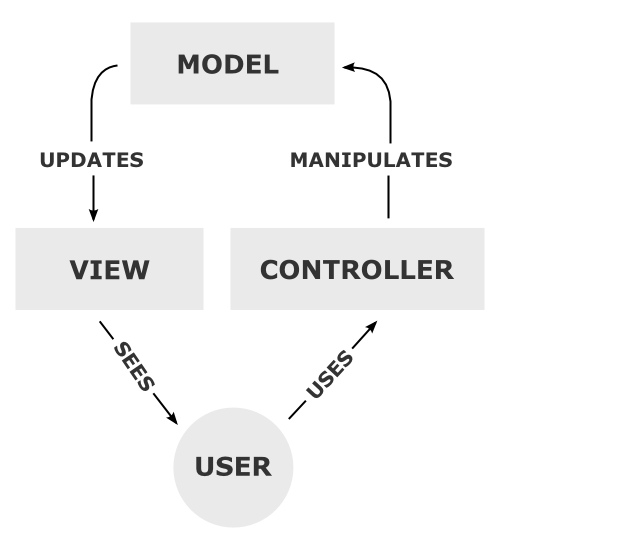
\includegraphics[width=.483\linewidth]{gfx/mvc}} \quad
        \subfloat[Model-View-ViewModel]
        {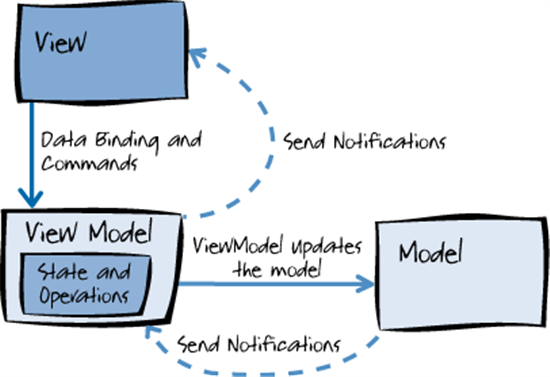
\includegraphics[width=.483\linewidth]{gfx/mvvm}} \\
        \caption[Common software architecture patterns]{Common software architecture patterns}\label{fig:sap}
\end{figure}  

\begin{table}[H]
    \myfloatalign
  \begin{tabularx}{\textwidth}{Xll} \toprule
    \tableheadline{} & \tableheadline{Xamarin} & \tableheadline{Titanium}\\ 
    \midrule
    Automated Builds & Possible & Possible\\
    Automated Tests & \ding{52} & \ding{56}\\
    Continuous Integration & Possible & Possible\\
    Version Control & \ding{52} & \ding{52}\\
    Architecture Pattern & MVVM & MVC (if using Alloy)\\
    %\midrule
    \bottomrule
  \end{tabularx}
  \caption[Feature support of Xamarin \& Titanium]{Feature support of Xamarin \& Titanium} \label{tab:maintain}
\end{table}

Another aspect of maintainability we haven't discussed yet is the amount of code produced when developing your application. If the framework you are using requires you to write less code to perform a given task, it can lead to a more maintainable application.

An important difference between Xamarin and Titanium is the way they handle the development of the \ac{UI} for each platform.

\begin{description}
\item[Xamarin] requires you to develop the \ac{UI} for each platform independently, which means that you will have to maintain a larger number of files.
\item[Titanium] gathers common elements from both supported platforms (iOS \& Android) and puts them in a common namespace, allowing you to reduce the amount of code necessary for simple \ac{UI} elements. Nonetheless, you still need to keep separate implementations for elements unique to each platform.
\end{description}
\vfill


\subsection{Language Features}

There are some language features that can lower the complexity of a program and ease the development process. This special features usually come from the standard library or each programming language. A very helpful feature are Lambdas, or anonymous functions, and Closures. Lambdas can help reduce the amount of code written, but can increase complexity and Closures provide better flexibility to your code.

Other features like \ac{LINQ} make it easier to process data from arrays, enumerable classes, XML documents, relational databases and third-party data sources.\footnote{\url{http://en.wikipedia.org/wiki/Language_Integrated_Query}} 

\begin{table}[H]
    \myfloatalign
  \begin{tabularx}{\textwidth}{Xll} \toprule
    \tableheadline{} & \tableheadline{Xamarin} & \tableheadline{Titanium}\\ 
    \midrule
    Closures \& Lambdas & \ding{52} & \ding{52}\\
    Garbage Collector & \ding{52} & Interpreter side\\
    LINQ & \ding{52} & \ding{56}\\
    \tableheadline{Supported platforms:} & &\\
    iOS & \ding{52} & \ding{52}\\
    Android & \ding{52} & \ding{52}\\
    Windows Phone & \ding{52} & \ding{56}\\
    Blackberry & \ding{56} & Limited Suport\\
    %\midrule
    \bottomrule
  \end{tabularx}
  \caption[Language Features of Xamarin \& Titanium]{Language Features of Xamarin \& Titanium} \label{tab:lang}
\end{table}



\subsection{Pricing Schemes}
As previously stated, most of the multi-platform frameworks are of the commercial nature. They require a monthly or yearly fee in order to give you access to all of their features. This is exactly the case with \textit{Xamarin} and \textit{Titanium}, there is however a huge difference between them.

Both frameworks provide a free package, \textsc{but} Xamarin's free package has some restrictions that Titanium's doesn't. In fact, most of Titanium's features can be used for free. Let's take a look at some of the features of each framework's free package:

\begin{table}[H]
    \myfloatalign
  \begin{tabularx}{\textwidth}{Xll} \toprule
    \tableheadline{} & \tableheadline{Xamarin} & \tableheadline{Titanium}\\ 
    \midrule
    Unlimited App Size & \ding{56} & \ding{52}\\
    Native Libraries & \ding{56} & Maybe\\ 
    Deploy to Device & \ding{52} & \ding{52}\\
    Deploy to App Stores & \ding{52} & \ding{52}\\
    Custom IDE & \ding{52} & \ding{52}\\
    Module Marketplace & \ding{52} & \ding{52}\\
    IDE Component Store Integration & \ding{52} & \ding{56}\\
    Pre-Built Cloud Services & \ding{56} & \ding{52}\\
    Support & Forums & Forums\\
    %\midrule
    \bottomrule
  \end{tabularx}
  \caption[Free features of Xamarin \& Titanium]{Free features of Xamarin \& Titanium} \label{tab:price}
\end{table}

The biggest and perhaps the only important limitations of Xamarin are the limited app size; for the starter package you are limited to 32KB of \ac{IL} code size; and the restriction of native libraries. You can't create a binding, or use an existing one, to connect to a library written in one of the platform's native language.\footnote{\url{http://xamarin.com/ios}} 

In order to lift these limitations you have to upgrade to at least the Indie Package, which costs \$299 per platform per year and is only licensed to an individual programmer. A company looking to give access to more than one developer needs to buy the Business Package for \$999 per developer per platform per year.\footnote{\url{https://store.xamarin.com/}}

Titanium also blocks some of its features behind a paywall, although these are most appealing to business and enterprise customers. There is no readily available information on Appcelerator's pricing scheme for Titanium. The only way of accessing the prices is to contact them with your information and have them send you a quote.\footnote{\url{http://www.appcelerator.com/plans-pricing/}}

\subsection{Community}
A thriving community is important if you ever run into a problem or issue that you have no idea how to solve. Thankfully both frameworks have been around for a long enough time to have built a good sized community. A simple Google search will yield you a vast number of already answered questions in StackOverflow\marginpar{StackOverflow is a Q\&A website designed to help programmers}. Both frameworks have dedicated tags that should help you find the questions and answers you are looking for.

Each company also provides its users with free forums where you can ask your questions and get help from members of the community. 





%*******************
\section{Conclusion}

To make the decision between frameworks a bit more mathematical, we will distribute points for each of the criteria previously mentioned and will be scoring each framework based on their features and shortcomings.

\begin{table}[H]
    \myfloatalign
  \begin{tabularx}{\textwidth}{Xll} \toprule
    \tableheadline{} & \tableheadline{Xamarin} & \tableheadline{Titanium}\\ 
    \midrule
    Productivity & 17/20 & 15/20\\
    Maintainability & 19/25 & 20/25\\ 
    Performance & 18.5/20 & 14/20\\
    Language Features & 9/10 & 7/10\\
    Pricing & 2.5/5 & 5/5\\
    Community & 17/20 & 16/20\\
    \midrule
    \textsc{Total} & 83/100 & 77/100 \\ %(1.426) (1.164)     
    \bottomrule
  \end{tabularx}
  \caption[Summary and Score for both Frameworks]{Summary and Score} \label{tab:score}
\end{table}

We devised the scoring scheme, so that the aspects we find most important would have higher possible scores. Based on what we tallied from all of the criteria we discussed in detail before, we can see that the difference between both frameworks is not that big. Both have their strengths and weaknesses, but they are completely capable of delivering a solid experience and producing great apps.

There is, however, a clear winner based on what we value the most. For all the reasons previously stated and based on the score above we choose \textsc{Xamarin} as the framework for the development of the MHM Job Portal Aggregator.
\newline


Now that we have chosen the right framework for our endeavor, we can take a look at the next piece of the puzzle. Before we can start with the development of the application, we still need to discuss a very important part of almost all current applications; a connection to the cloud. 

In the next part we will discuss what the cloud actually is, how it comes into play with mobile applications and why so may companies are investing Millions of Dollars in cloud technology. 